\documentclass[border=3pt,tikz]{standalone}
% Shared look for every TikZ figure in these notes.
% Included by each standalone figure file; also keeps the figures consistent
% with the colours used in the PDF and on the website.

\usepackage{tikz}
\usepackage{pgfplots}
\pgfplotsset{compat=1.18}
\usetikzlibrary{arrows.meta, decorations.markings, decorations.pathmorphing,
                patterns, calc, positioning}
\usepackage{amsmath}

% Series colours are the three validated categorical slots also used by the
% interactive widgets, so a path drawn in the printed notes and the same path on
% the website are the same colour. They clear the colour-vision-deficiency and
% contrast checks as a set; every path is direct-labelled as well, so colour is
% never the only thing carrying identity.
\definecolor{duPurple}{HTML}{68246D}
\definecolor{duBlue}{HTML}{2A78D6}
\definecolor{duRed}{HTML}{EB6834}
\definecolor{duGreen}{HTML}{1BAF7A}
\definecolor{duGrey}{HTML}{6B6B6B}

\tikzset{
  axisline/.style   = {-{Stealth[length=3mm]}, line width=0.7pt, black},
  path1/.style      = {duBlue,   line width=1.1pt},
  path2/.style      = {duRed,    line width=1.1pt},
  path3/.style      = {duGreen,  line width=1.1pt},
  statedot/.style   = {circle, fill=black, inner sep=1.4pt},
  arrowhead/.style  = {decoration={markings,
                        mark=at position #1 with {\arrow{Stealth[length=2.6mm]}}},
                       postaction={decorate}},
  lbl/.style        = {font=\small},
  slbl/.style       = {font=\footnotesize, duGrey},
  workfill/.style   = {duPurple, opacity=0.16},
}

\begin{document}
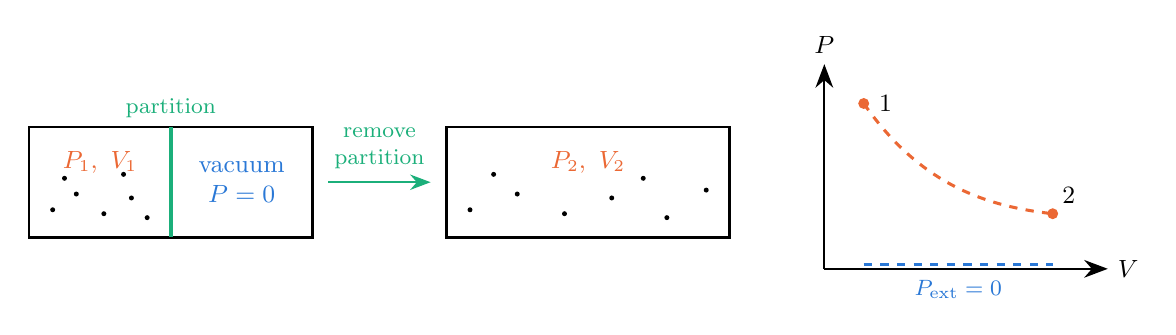
\begin{tikzpicture}
  % before: gas | vacuum
  \draw[line width=1pt] (0,0) rectangle (3.6,1.4);
  \draw[line width=1.4pt, duGreen] (1.8,0) -- (1.8,1.4);
  \node[lbl, duRed] at (0.9,0.95) {$P_1,\ V_1$};
  \foreach \x/\y in {0.3/0.35,0.6/0.55,0.95/0.3,1.3/0.5,1.5/0.25,0.45/0.75,1.2/0.8} \fill (\x,\y) circle (0.9pt);
  \node[lbl, duBlue, align=center] at (2.7,0.7) {vacuum\\$P = 0$};
  \node[slbl, duGreen, above] at (1.8,1.4) {partition};
  \draw[-{Stealth[length=2.6mm]}, line width=0.8pt, duGreen] (3.8,0.7) -- (5.1,0.7);
  \node[slbl, duGreen, align=center, above] at (4.45,0.75) {remove\\partition};
  % after
  \begin{scope}[shift={(5.3,0)}]
    \draw[line width=1pt] (0,0) rectangle (3.6,1.4);
    \node[lbl, duRed] at (1.8,0.95) {$P_2,\ V_2$};
    \foreach \x/\y in {0.3/0.35,0.9/0.55,1.5/0.3,2.1/0.5,2.8/0.25,3.3/0.6,2.5/0.75,0.6/0.8} \fill (\x,\y) circle (0.9pt);
  \end{scope}
  % P-V diagram
  \begin{scope}[shift={(10.1,-0.4)}]
    \draw[axisline] (0,0) -- (3.6,0) node[right, lbl] {$V$};
    \draw[axisline] (0,0) -- (0,2.6) node[above, lbl] {$P$};
    \draw[path2, dashed] (0.5,2.1) .. controls (1.2,1.1) and (2.0,0.8) .. (2.9,0.7);
    \node[circle, fill=duRed, inner sep=1.4pt] at (0.5,2.1) {};
    \node[circle, fill=duRed, inner sep=1.4pt] at (2.9,0.7) {};
    \node[lbl, right=2pt] at (0.5,2.1) {1};
    \node[lbl, above right=0pt] at (2.9,0.7) {2};
    \draw[path1, dashed] (0.5,0.06) -- (2.9,0.06);
    \node[slbl, duBlue, below] at (1.7,-0.02) {$P_\text{ext} = 0$};
  \end{scope}
\end{tikzpicture}
\end{document}
